% \begin{columns}[T]
%   \begin{column}{0.45\textwidth}
%   \end{column}
%   \begin{column}{0.45\textwidth}
%   \end{column}
% \end{columns}

\section{Prototype tests and results}
\subsection{Preliminary tests at IRMA}
\begin{frame}[t]
  \frametitle{Tests of the silicon detector at IRMA}
  \begin{columns}
    \begin{column}{0.45\textwidth}
      IRMA (CSNSM/CNRS/Orsay):
      \begin{itemize}
        \item Ion implantation source
        \item $5$ to $190\,\mathrm{keV}$
        \item Many species
      \end{itemize}
      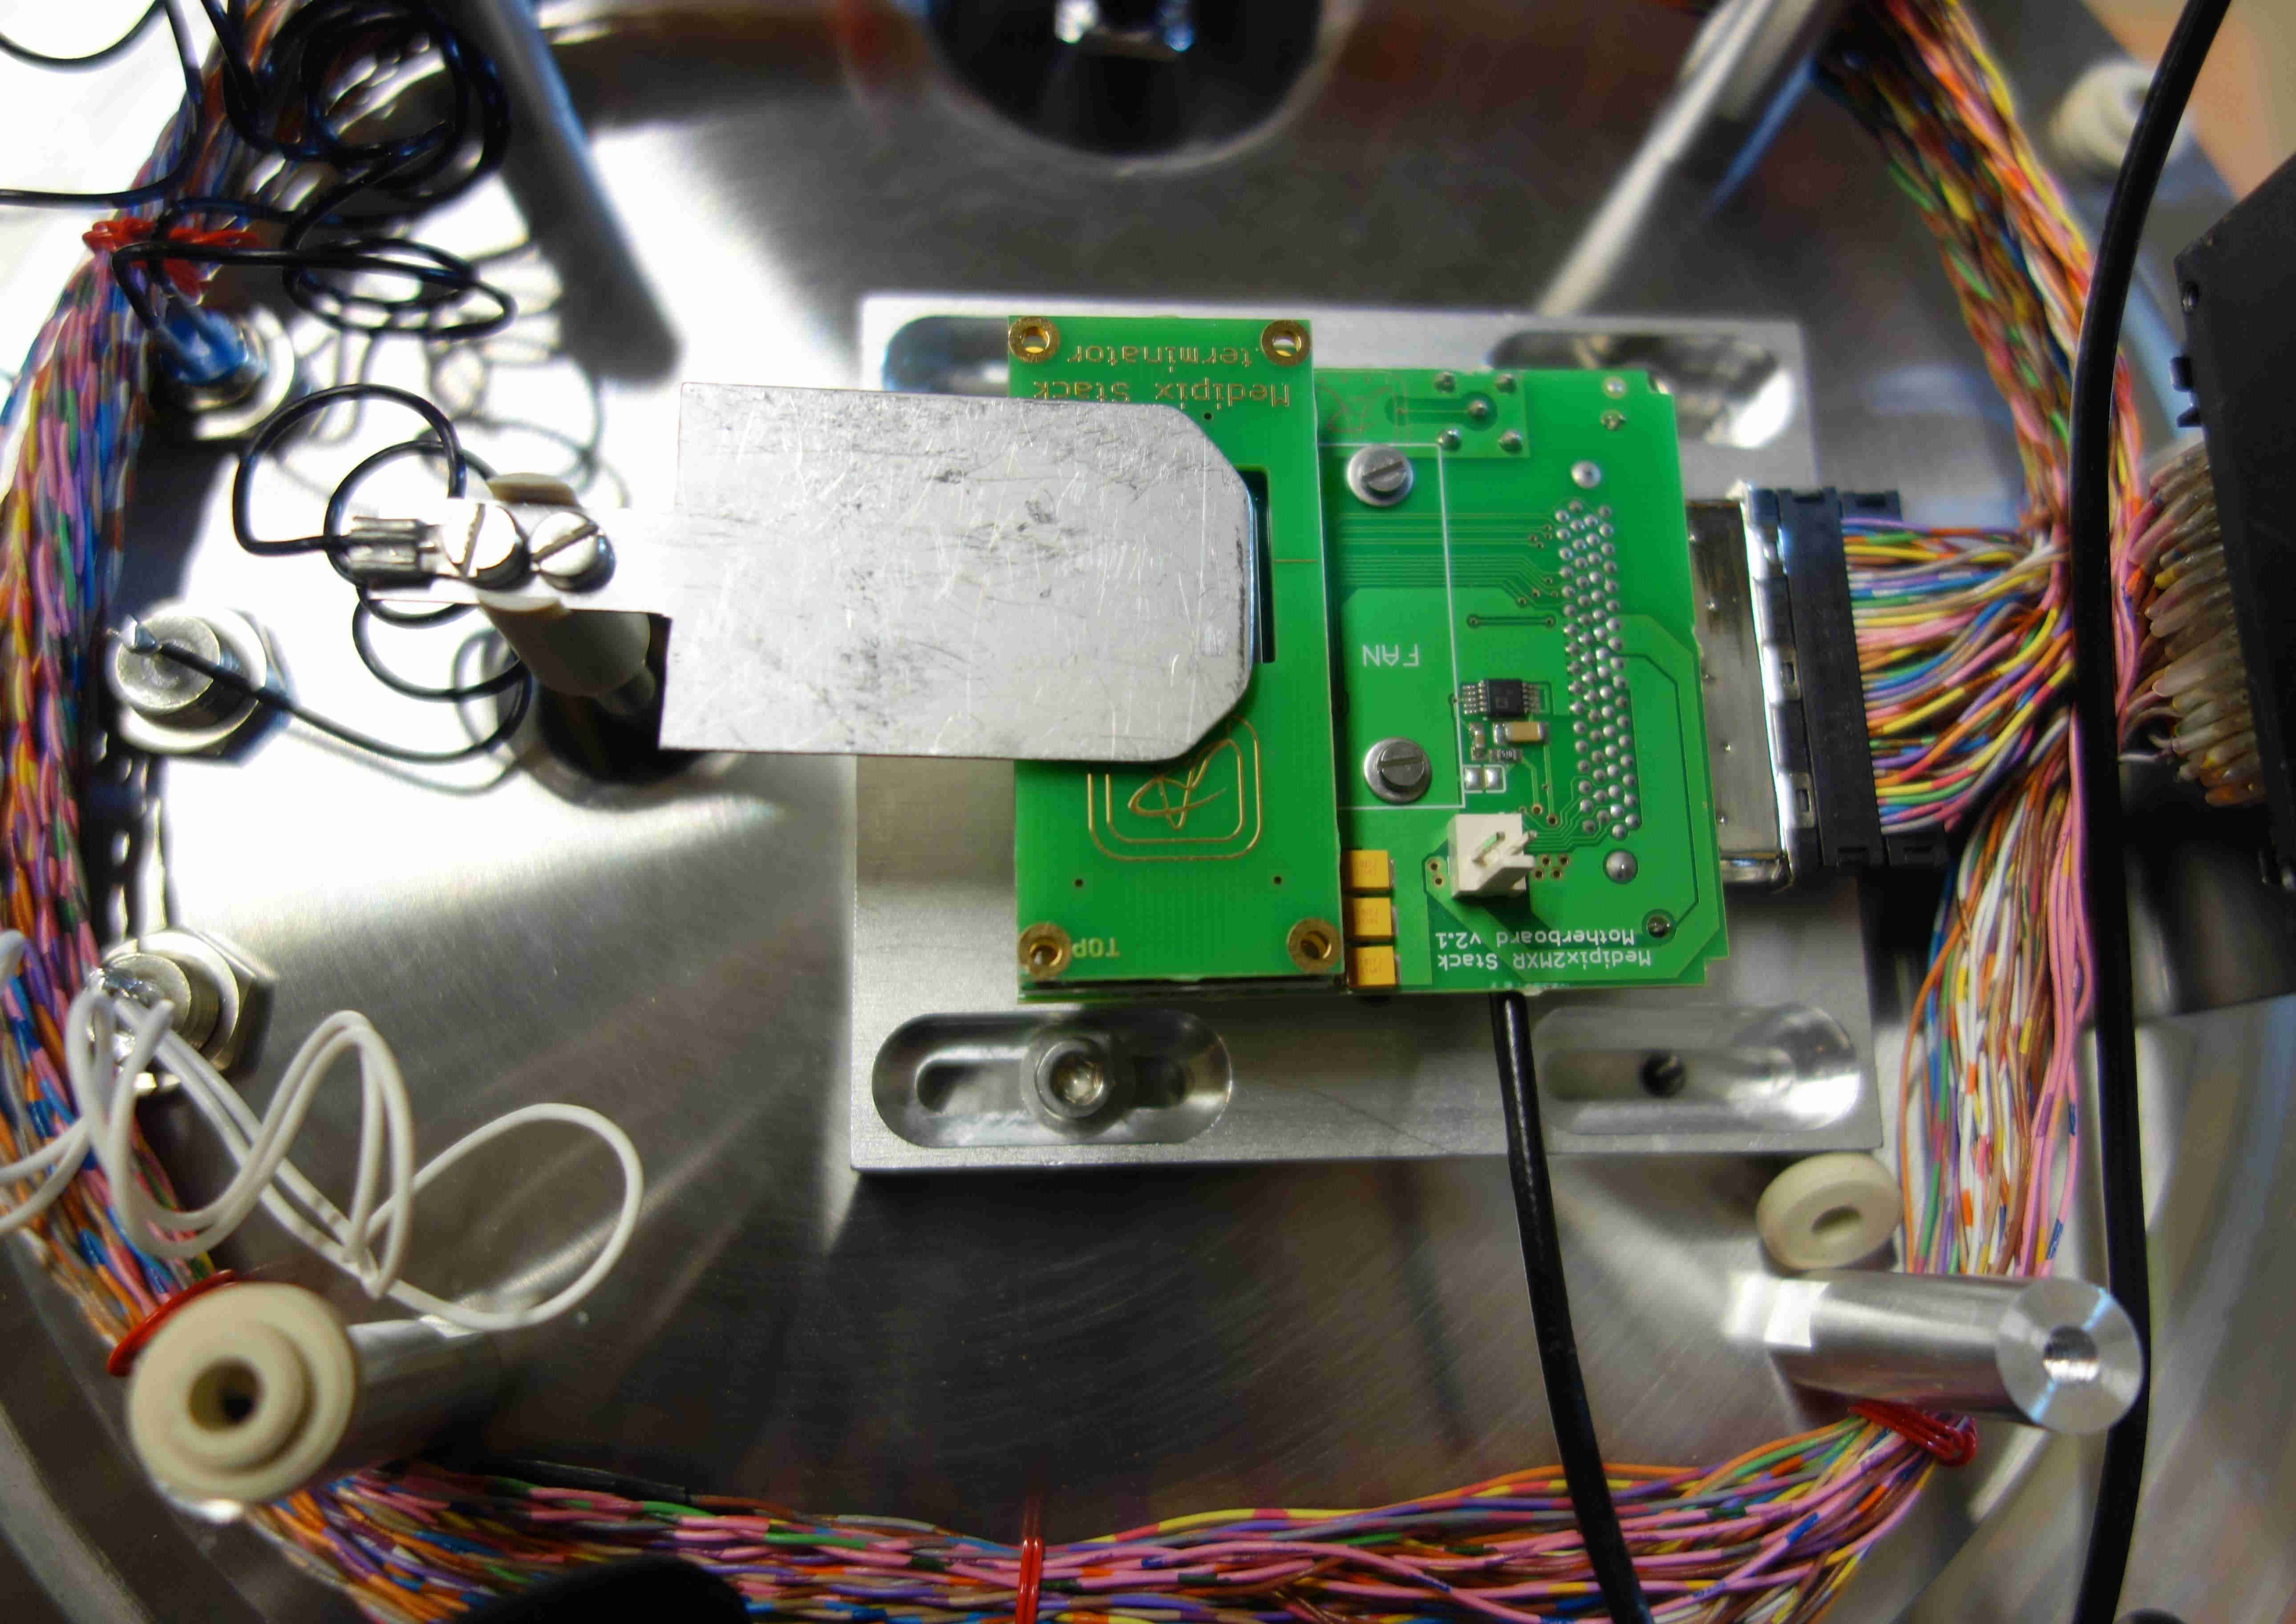
\includegraphics[width=\textwidth]{04_Test/fig/fig000_IRMA_setup01.jpg}
    \end{column}
    \begin{column}{0.45\textwidth}
      \begin{columns}
        \begin{column}{0.45\textwidth}
          \centering
          $15\,\mathrm{keV}$
          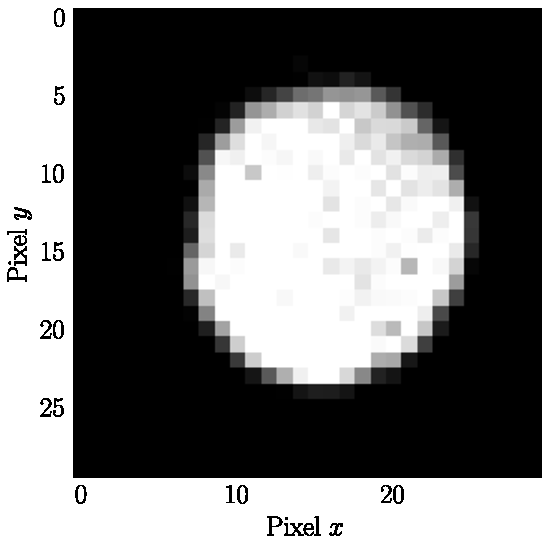
\includegraphics[width=0.8\textwidth]{04_Test/fig/fig000_IRMA_15keV_svg-tex.pdf}
        \end{column}
        \begin{column}{0.45\textwidth}
          \centering
          $12\,\mathrm{keV}$
          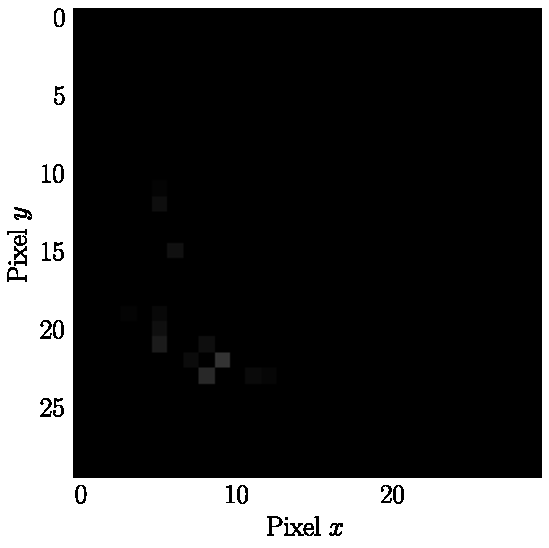
\includegraphics[width=0.8\textwidth]{04_Test/fig/fig000_IRMA_12keV_svg-tex.pdf}
        \end{column}
      \end{columns}
      \centering
      Damage after irradiation
      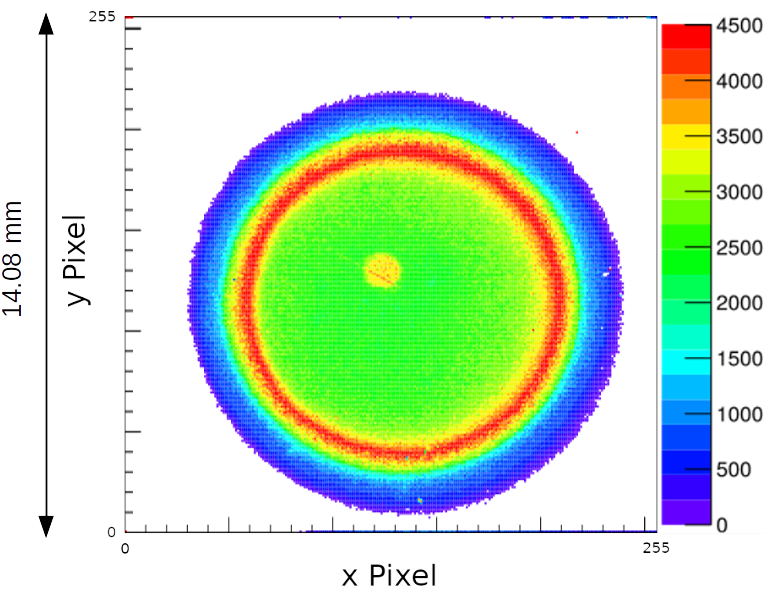
\includegraphics[width=0.8\textwidth]{04_Test/fig/fig000_IRMA_damage5.png}
    \end{column}
  \end{columns}
  \begin{alertblock}{Interesting results}
    But required more investigations $\rightarrow$ not possible with the given schedule.
  \end{alertblock}
\end{frame}

\subsection{IPM testbench}
\begin{frame}[t]
  \frametitle{IPM prototypes}
  \begin{columns}
    \begin{column}{0.45\textwidth}
      \begin{block}{Prototype characteristics}
        \begin{itemize}
          \item Cage: $10\times10\times10\,\mathrm{cm^3}$
          \item Active area: $4\times2\,\mathrm{cm^2}$
          \item The readout can be easily changed.
        \end{itemize}
      \end{block}

      \begin{block}{Vacuum compliant materials}
        \begin{itemize}
          \item Steel and copper
          \item Macor
          \item PEEK
          \item Ceramic PCB
        \end{itemize}
      \end{block}

    \end{column}
    \begin{column}{0.45\textwidth}
      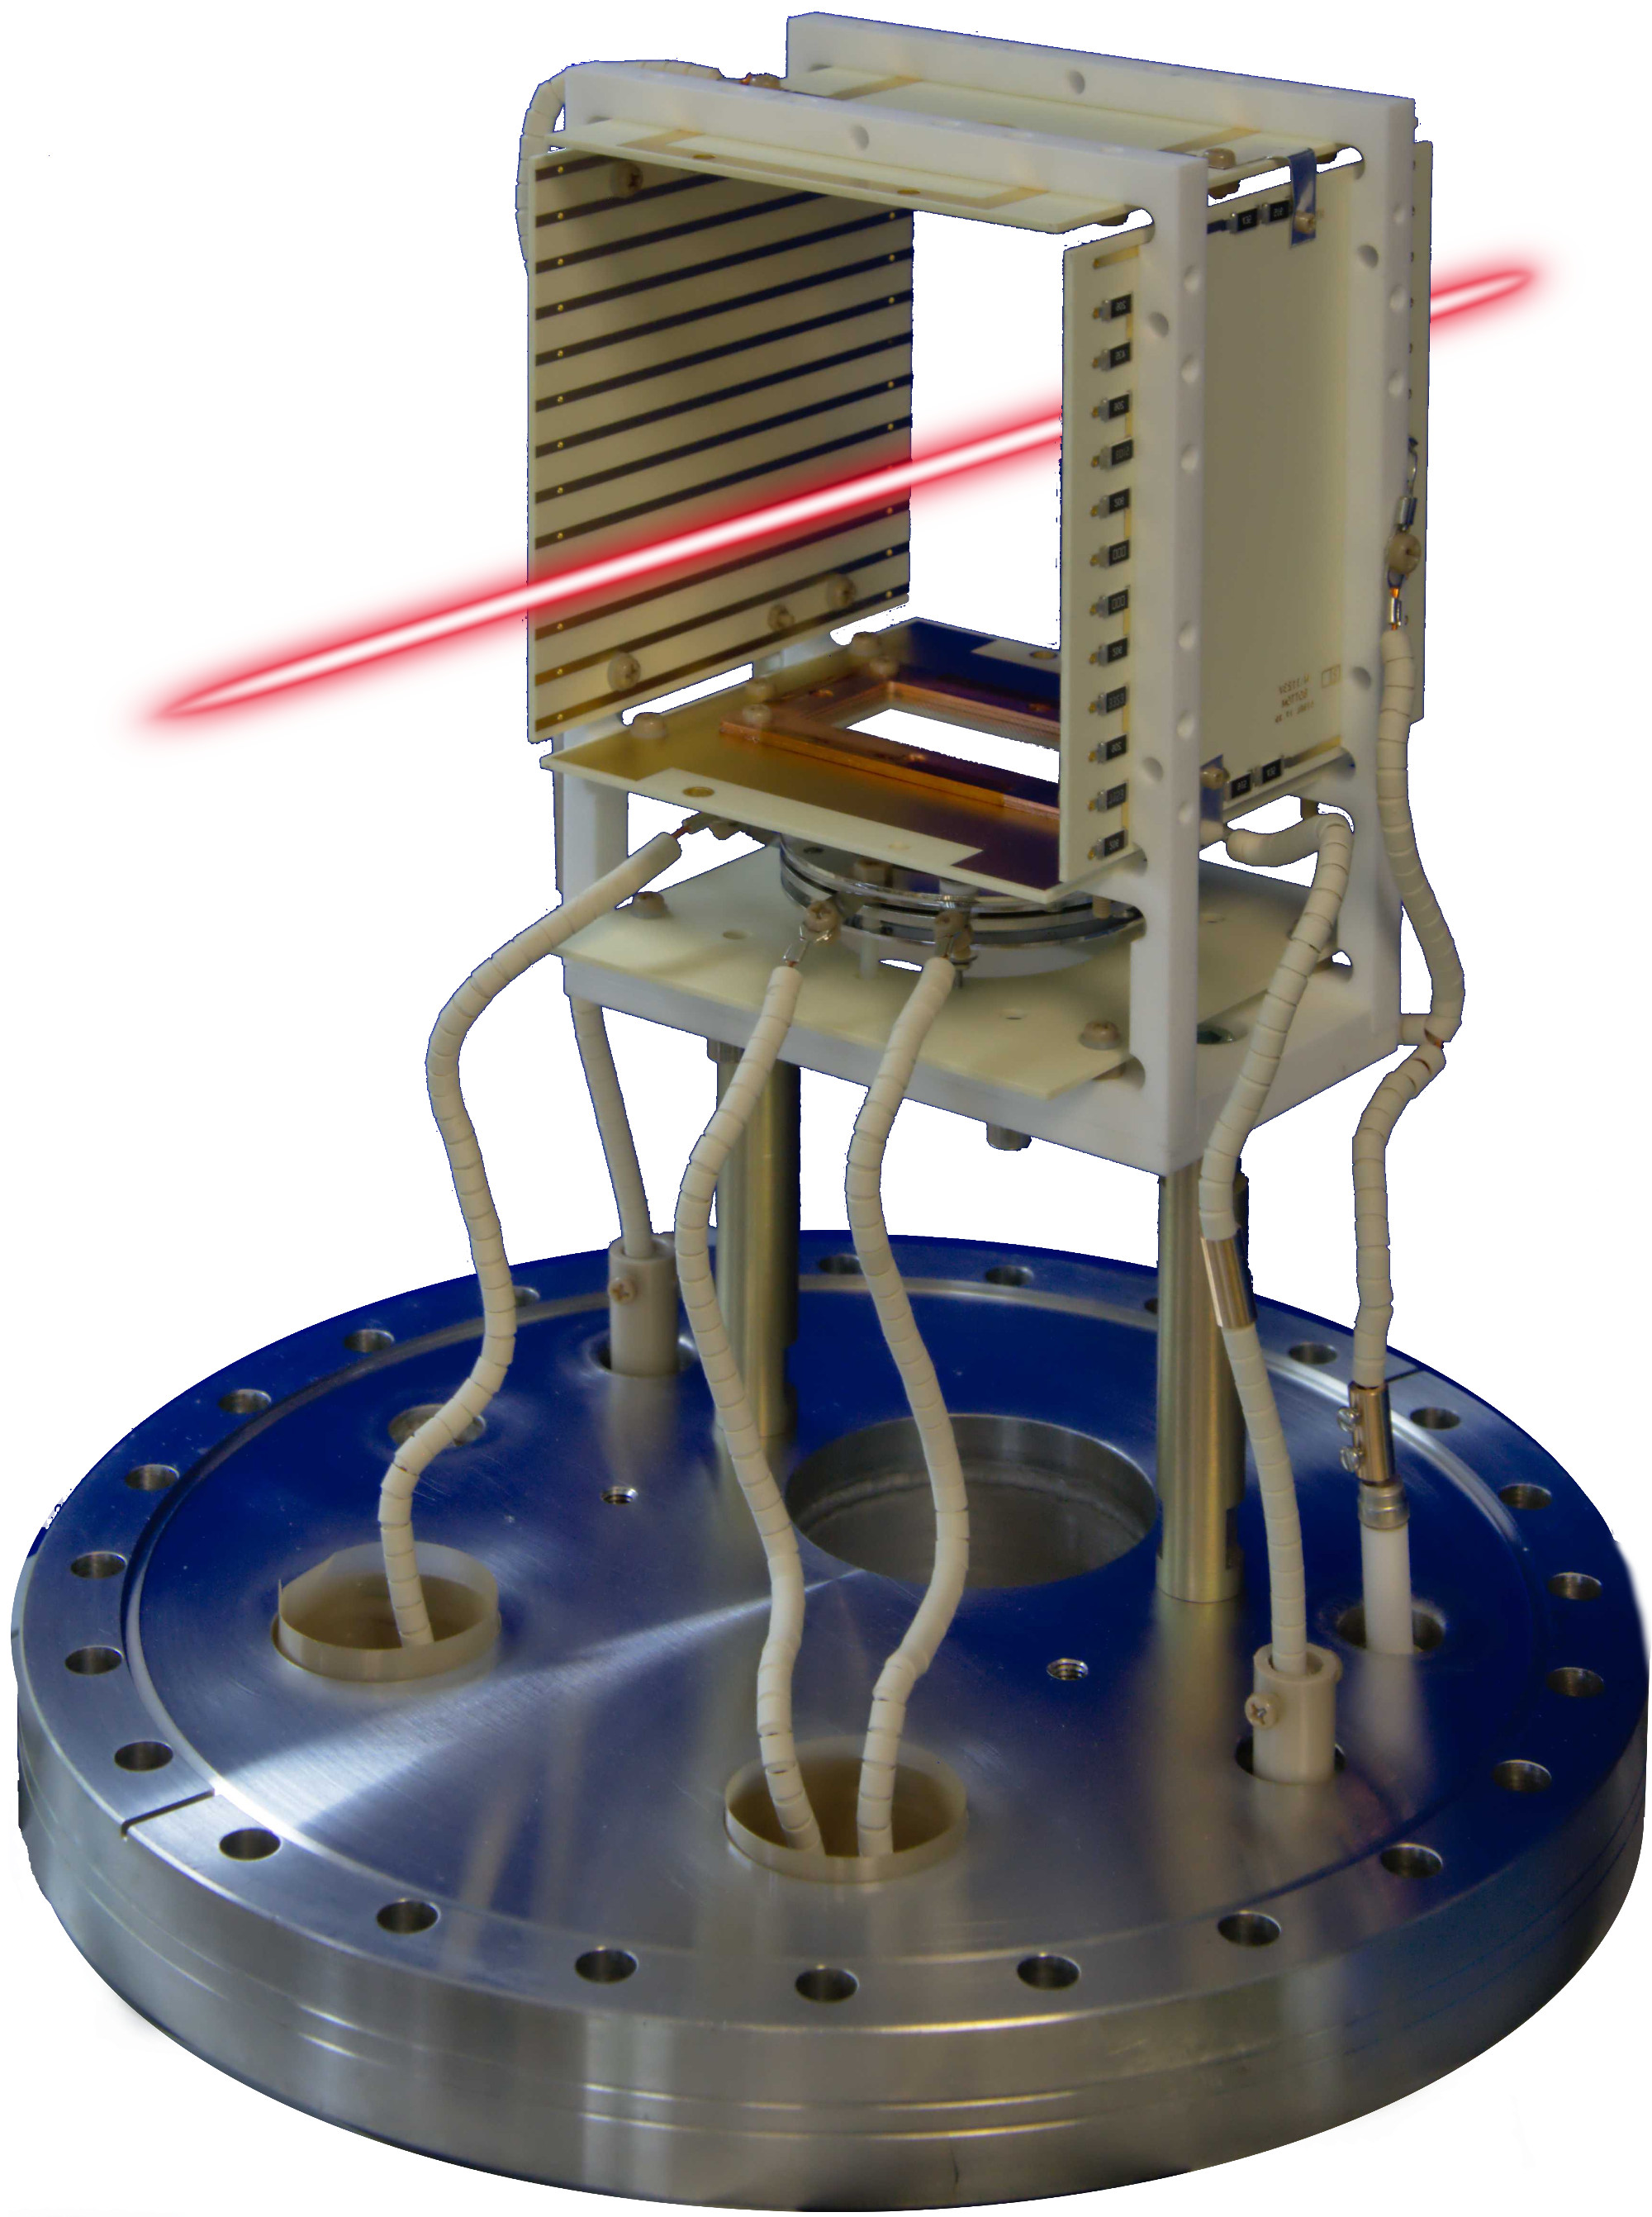
\includegraphics[width=\textwidth]{04_Test/fig/fig000_IPM_photo2}
    \end{column}
  \end{columns}
\end{frame}

\begin{frame}[t]
  \frametitle{IPM test bench}
  A dedicated test bench has been developed:
  \begin{columns}[T]
    \begin{column}{0.60\textwidth}
      \begin{center}
        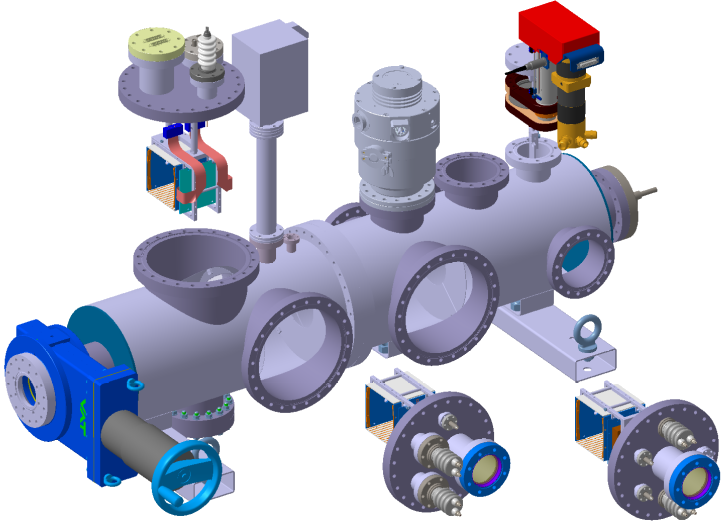
\includegraphics[width=0.8\textwidth]{04_Test/fig/fig000_Testbench2.png}
      \end{center}
    \end{column}

    \begin{column}{0.30\textwidth}
      \begin{block}{Integration}
        \begin{itemize}
          \item Vacuum:
                \begin{itemize}
                  \item Cleaning
                  \item Leak test
                  \item Baking
                \end{itemize}
          \item Control system:
                \begin{itemize}
                  \item HV
                  \item Camera
                \end{itemize}
        \end{itemize}
      \end{block}
    \end{column}
  \end{columns}
  \begin{columns}[T]
    \begin{column}{0.45\textwidth}
      \begin{block}{Upstream}
        \begin{itemize}
          \item Mimic ESS vacuum chamber.
          \item 2 slots for IPM prototypes.
        \end{itemize}
      \end{block}
    \end{column}

    \begin{column}{0.45\textwidth}
      \begin{block}{Downstream}
        \begin{itemize}
          \item Extension adding more slots.
          \item 1 slot for an IPM prototype.
          \item 2 slots for reference measurements.
        \end{itemize}
      \end{block}
    \end{column}
  \end{columns}

\end{frame}

\subsection{IPHI}
\begin{frame}[t]
  \frametitle{IPHI}
  \begin{block}{Injector of Proton for High Intensity}
    IPHI is a high intensity $3\,\mathrm{MeV}$ proton accelerator at DACM/IRFU/CEA Saclay. IPHI can be seen as the 20 first meters of ESS.
  \end{block}
  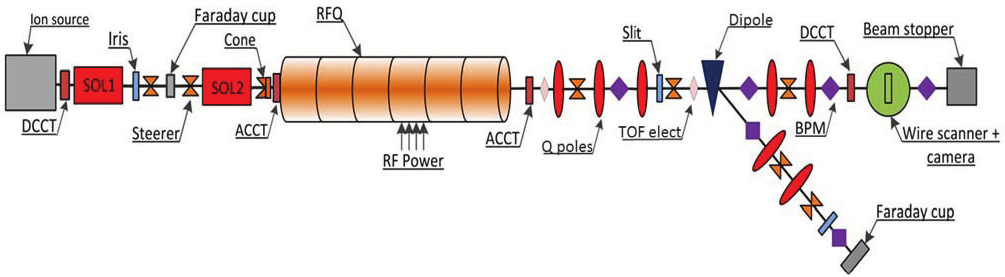
\includegraphics[width=1\textwidth]{04_Test/fig/fig000_IPHI_view.png}
  \begin{tabularx}{\linewidth}{XXX}
    \toprule
                         & IPHI accelerator                                  & ESS accelerator                \\
    \midrule
    Energy               & $3\,\mathrm{MeV}$                                 & $2\,\mathrm{GeV}$              \\
    Max current          & $0.5-100\,\mathrm{mA}$                            & $62.5\,\mathrm{mA}$            \\
    Max pulse duration   & $>100\,\mathrm{\mu s}$ up to CW                   & $2.86\,\mathrm{ms}$            \\
    Max pulse repetition & -                                                 & $14\,\mathrm{Hz}$              \\
    Vacuum range         & $5\cdot10^{-7}$ to $1\cdot10^{-8}\,\mathrm{mbar}$ & $1\cdot10^{-9}\,\mathrm{mbar}$ \\
    \bottomrule
  \end{tabularx}
\end{frame}

\begin{frame}[t]
  \frametitle{IPHI test campaign}
  \begin{block}{Goals:}
    \begin{itemize}
      \item Characterize our prototypes and readouts.
      \item Find flaws in the IPMs.
    \end{itemize}
  \end{block}
  \begin{columns}[T]
    \begin{column}{0.45\textwidth}
      \centering
      IPHI installation
      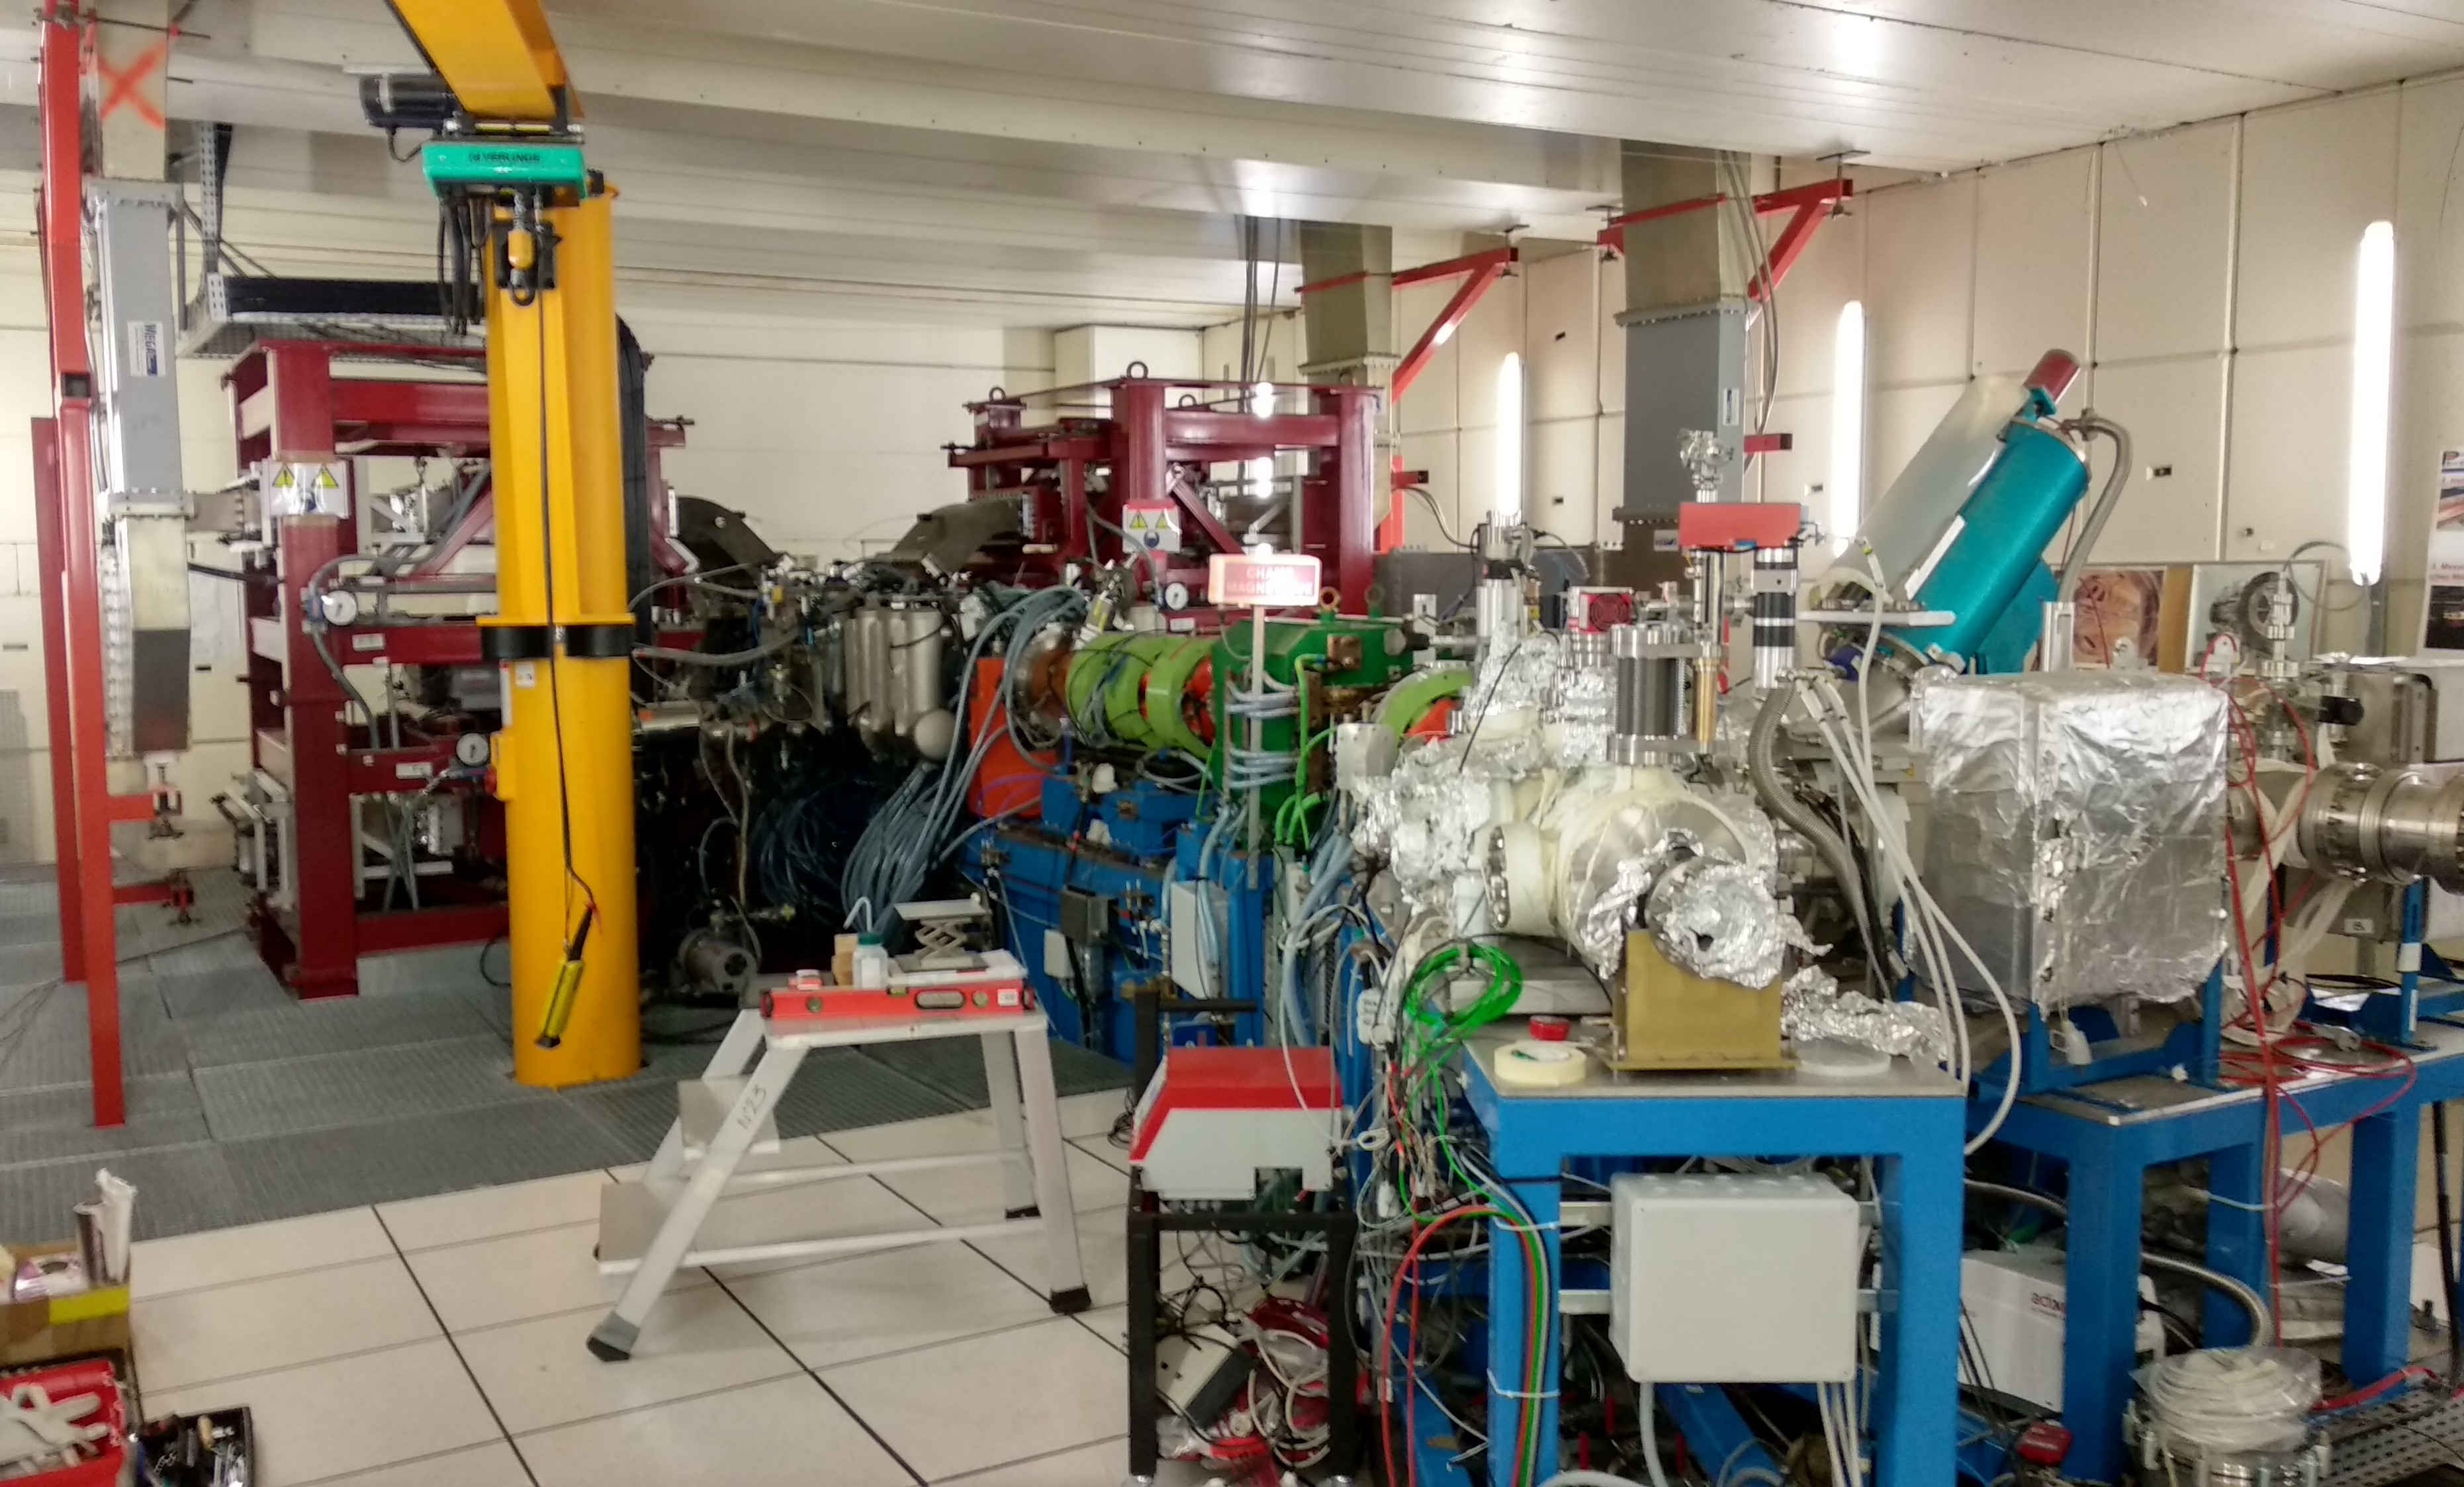
\includegraphics[width=1\textwidth]{04_Test/fig/fig000_IPHI_tb1.jpg}
    \end{column}
    \begin{column}{0.45\textwidth}
      \centering
      IPM test bench at IPHI
      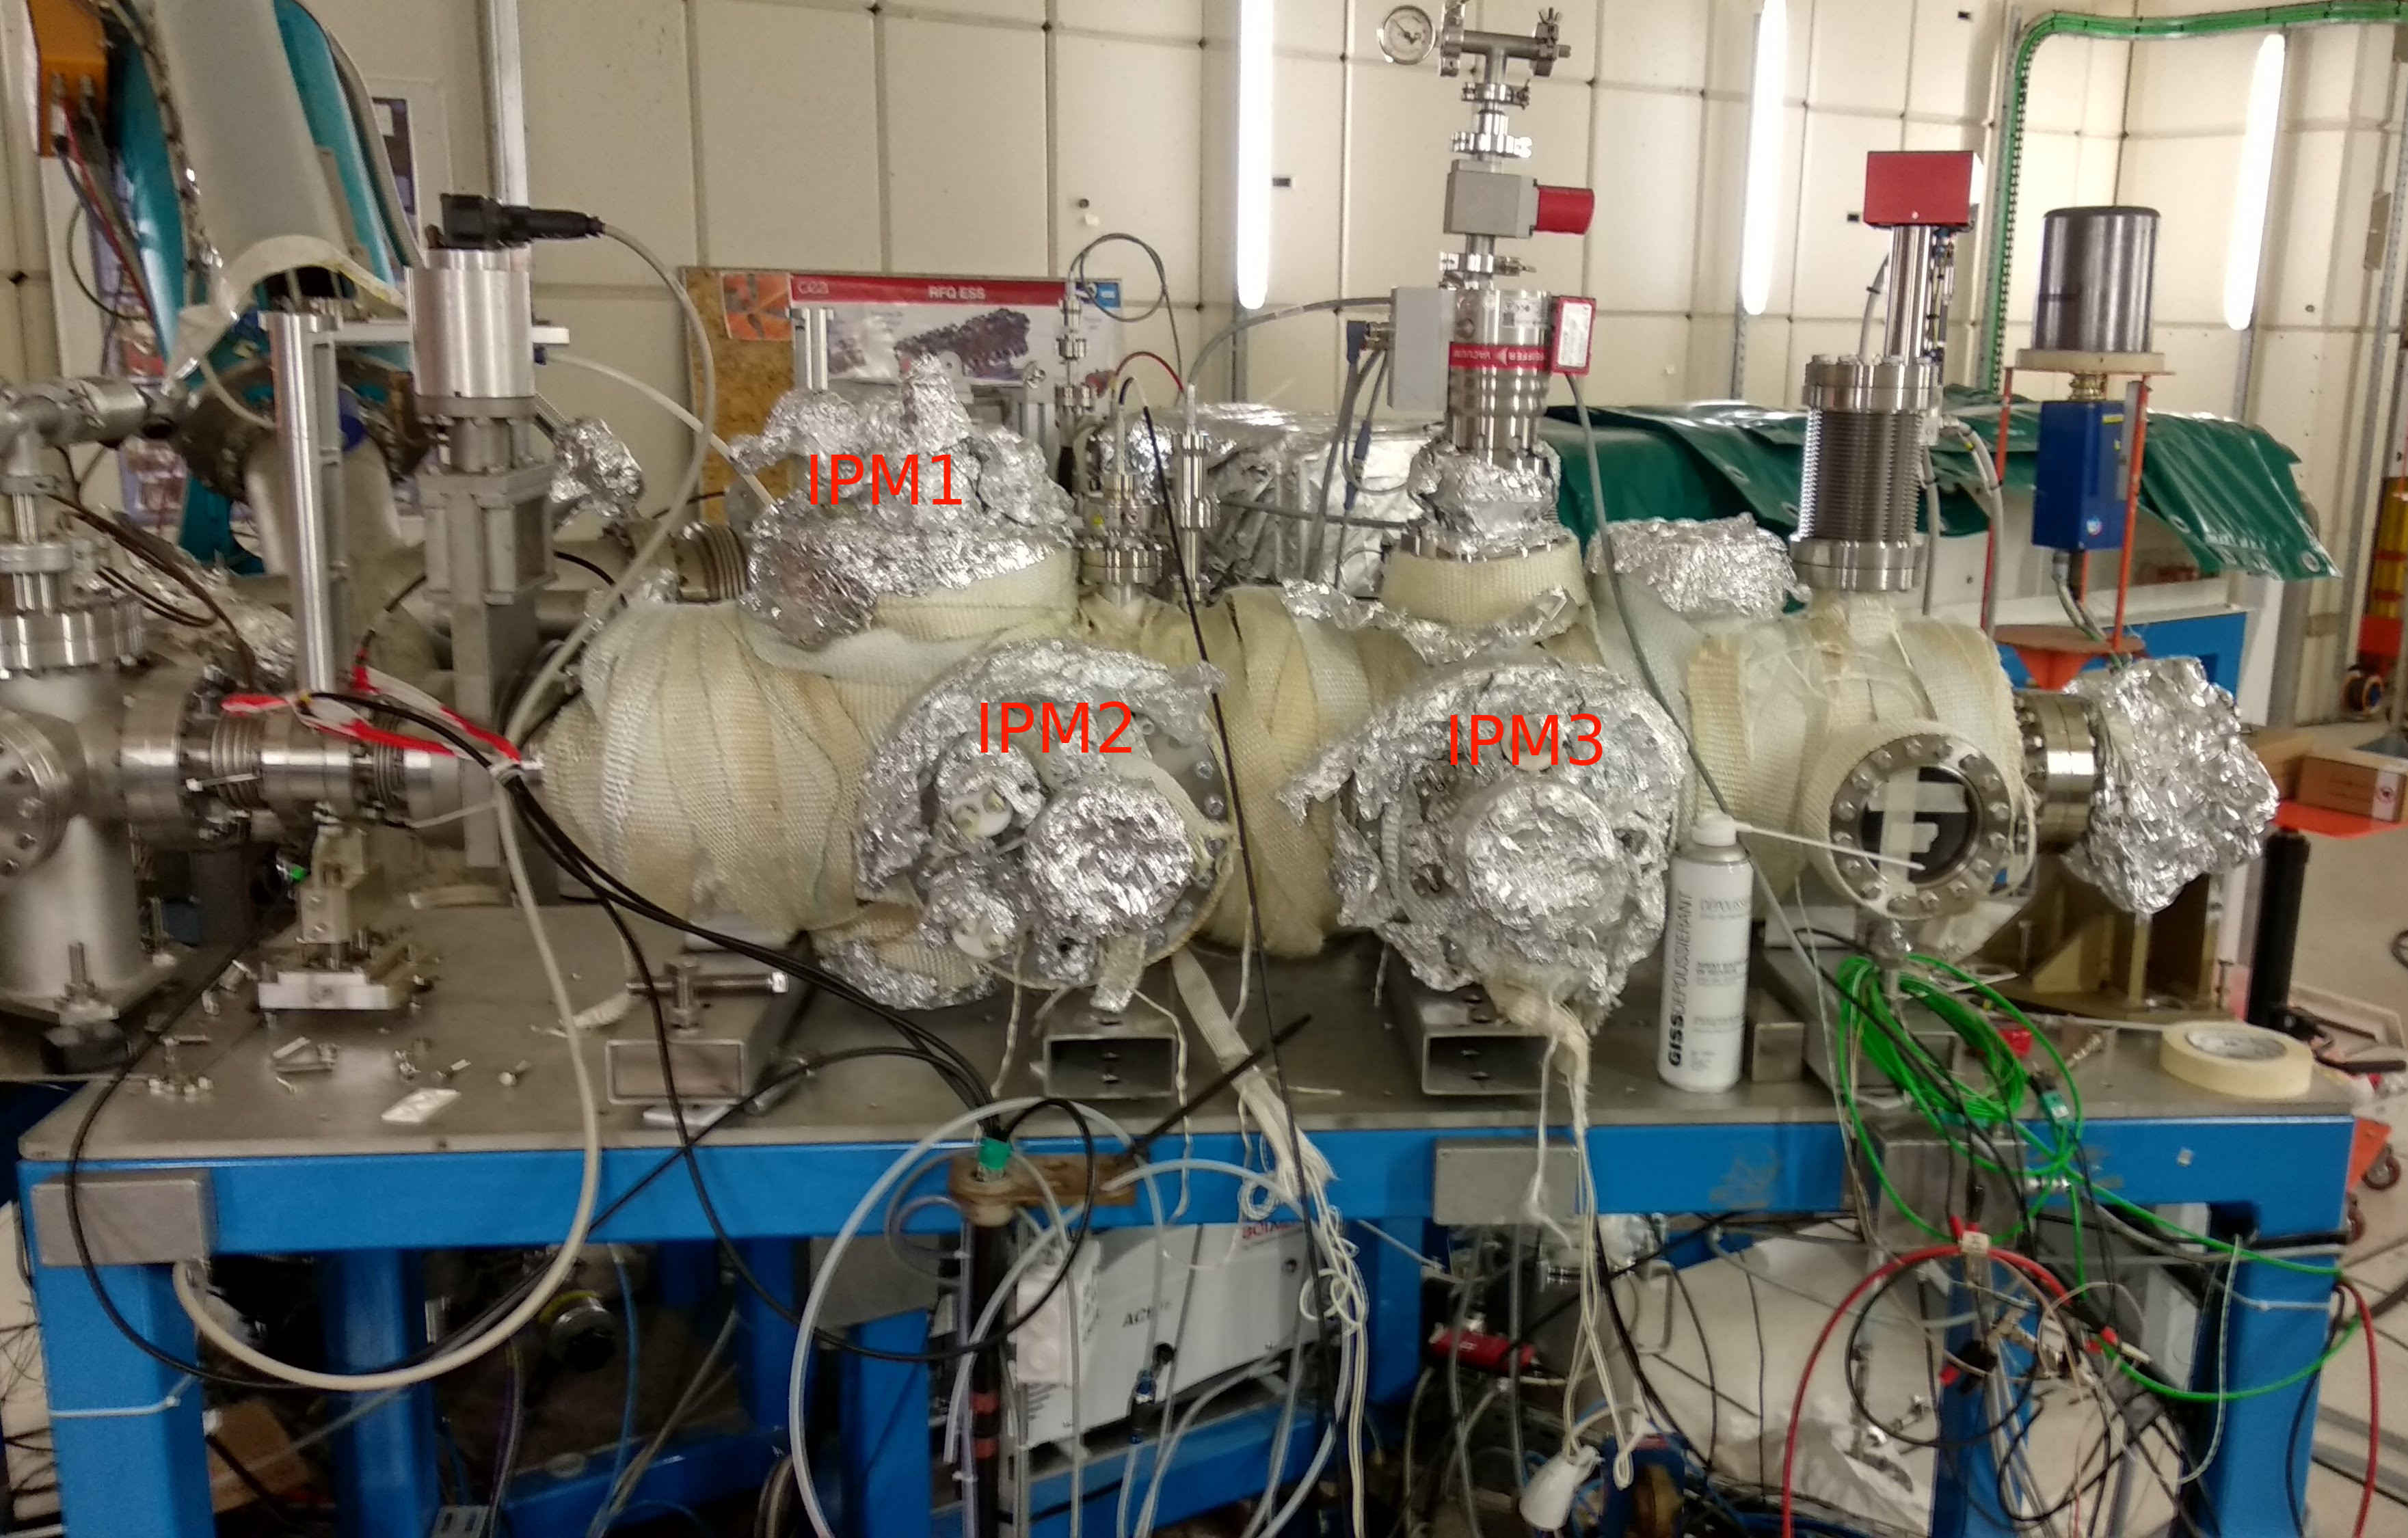
\includegraphics[width=1\textwidth]{04_Test/fig/fig000_IPHI_tb2.jpg}
    \end{column}
  \end{columns}
  \begin{block}{Two campaigns:}
    \begin{itemize}
      \item First campaign: Setup and first tests.
      \item Second campaign: improved prototypes, check limits.
    \end{itemize}
  \end{block}
\end{frame}

\subsection{Results}
\begin{frame}[t]
  \frametitle{Processing data from IPMs}
  \begin{columns}[T]
    \begin{column}{0.45\textwidth}
      \begin{block}{Processing data from camera}
        \begin{enumerate}
          \item Crop image to ROI
          \item Remove dead pixels
          \item Filtering
          \item Sum along longitudinal direction
        \end{enumerate}
      \end{block}
      \begin{center}
        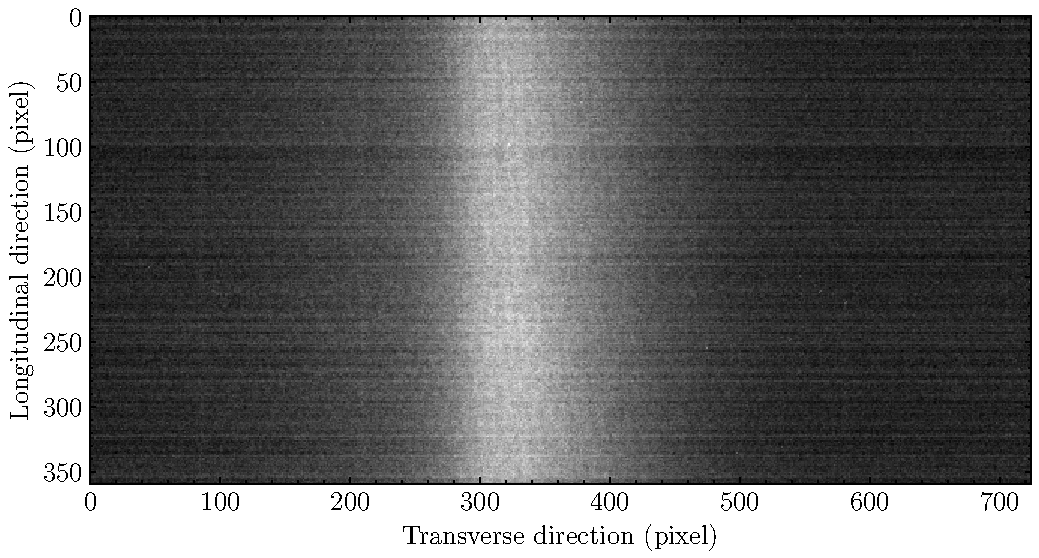
\includegraphics[width=1\textwidth]{04_Test/fig/fig000_image_beam}
        \begin{tikzpicture}[every node/.style={single arrow, draw=none, rotate=90}]
          \node [fill=red!50] {Beam};
        \end{tikzpicture}
      \end{center}
    \end{column}
    \begin{column}{0.45\textwidth}
      \begin{block}{Processing data from strips}
        \begin{enumerate}
          \item Remove pedestals
          \item FFT Filtering
          \item Event finding with threshold
          \item Check multiplicity on several strips
        \end{enumerate}
      \end{block}
      \only<1>{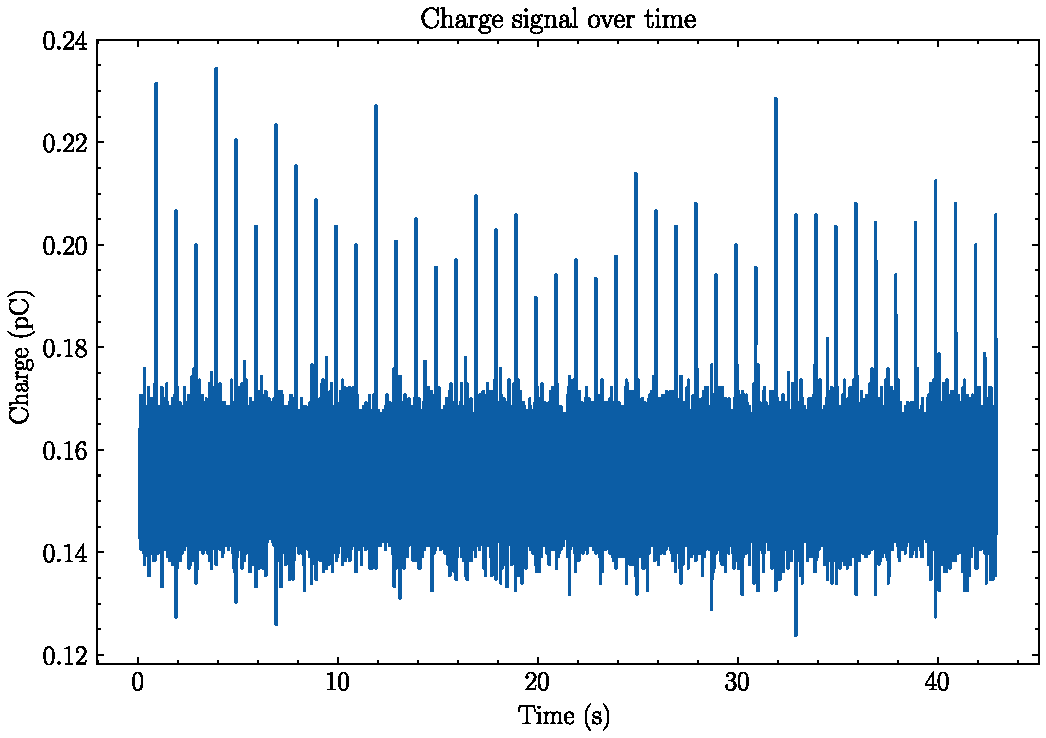
\includegraphics[width=1\textwidth]{04_Test/fig/fig000_strips_signal}}
      \only<2>{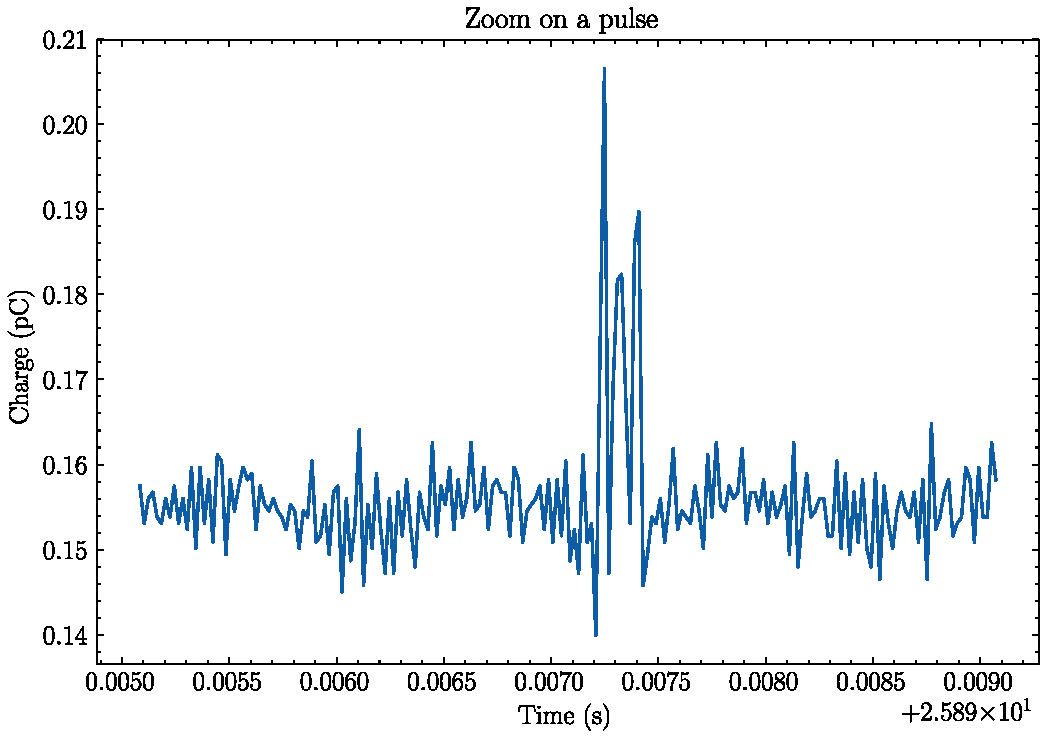
\includegraphics[width=1\textwidth]{04_Test/fig/fig000_strips_signal_b}}
    \end{column}
  \end{columns}
\end{frame}

\begin{frame}[t]
  \frametitle{Profile comparison between IPMs}
  \begin{block}{Same pulse measuremement with strips and MCP}
    $i_{beam}=26\,\mathrm{mA}$ and $t_{pulse}=190\,\mathrm{\mu s}$
  \end{block}
  \begin{center}
    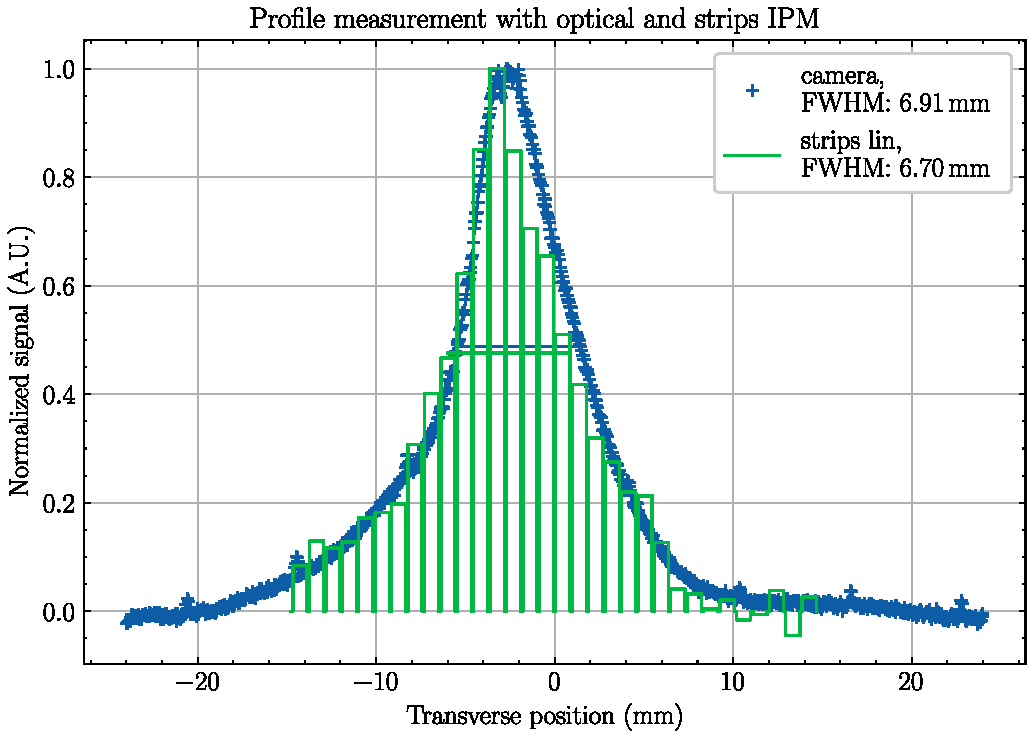
\includegraphics[width=0.75\textwidth]{04_Test/fig/fig000_MCP_strip}
  \end{center}
\end{frame}

\begin{frame}[t]
  \frametitle{Comparison with IPHI diagnostic}
  \begin{block}{Comparison with other diagnostic devices}
    No profile monitor available at IPHI $\implies$ compare other quantities
  \end{block}
  \begin{columns}[T]
    \begin{column}{0.45\textwidth}
      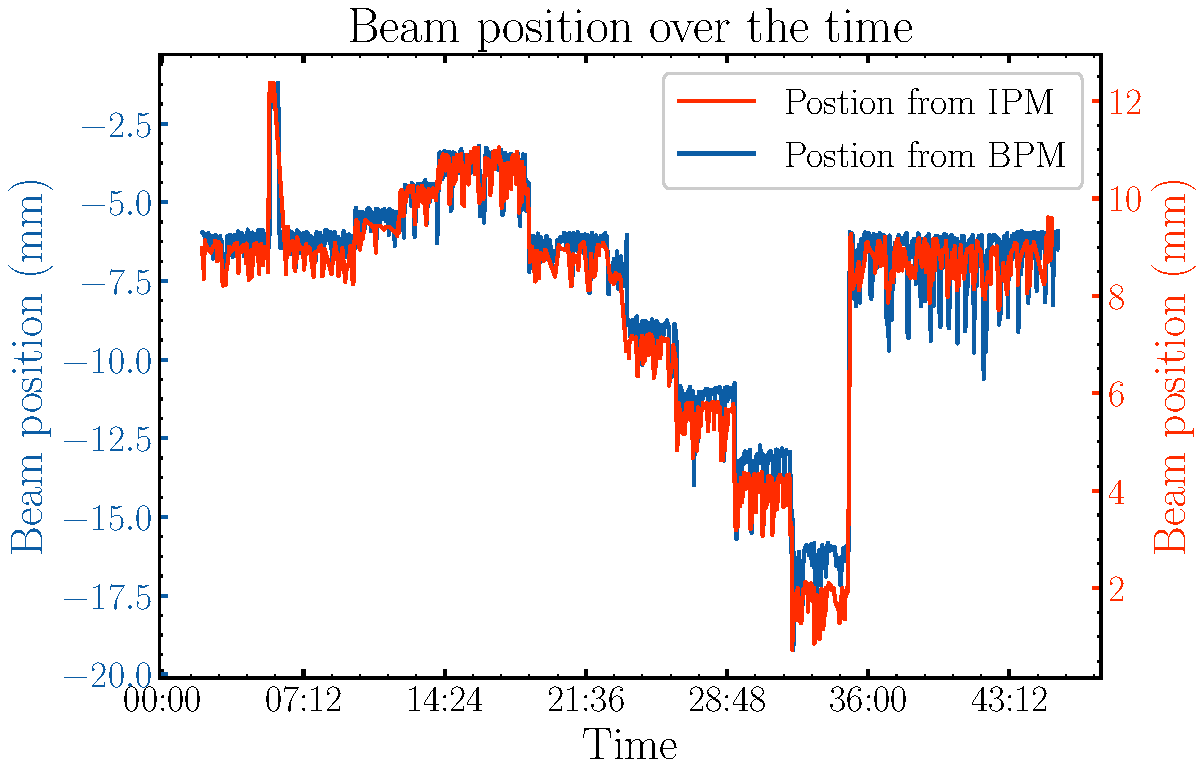
\includegraphics[width=1.14\textwidth]{04_Test/fig/fig000_beam_car_a}
    \end{column}
    \begin{column}{0.45\textwidth}
      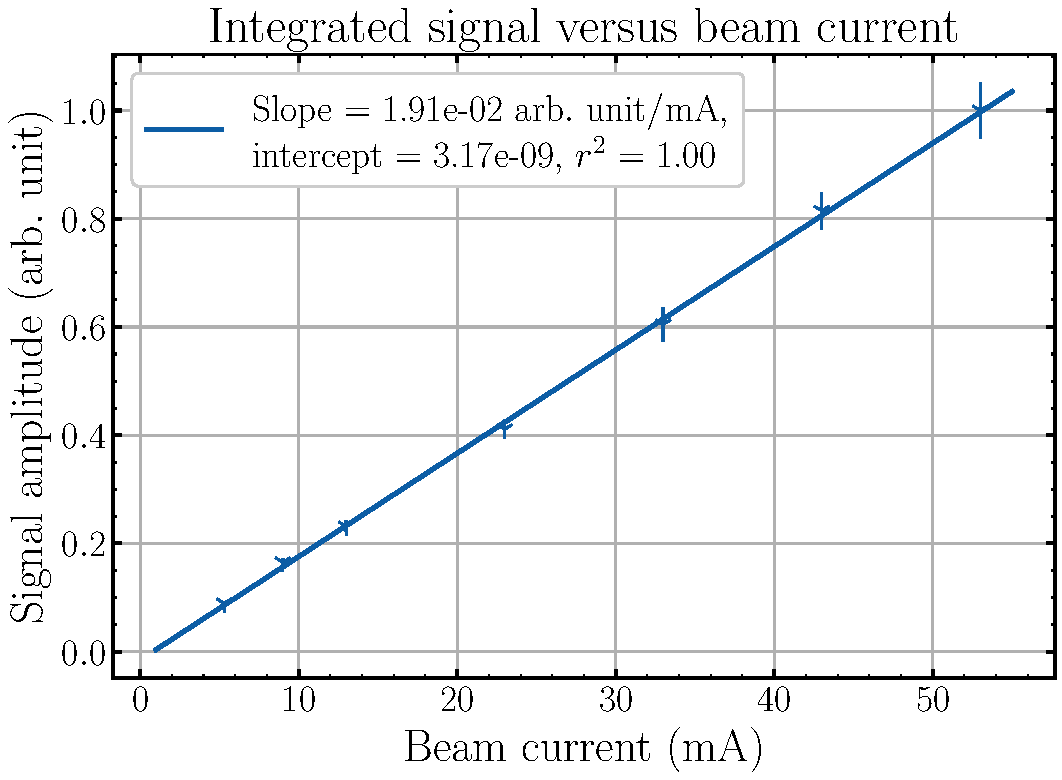
\includegraphics[width=1\textwidth]{04_Test/fig/fig000_current_sweep_a}
    \end{column}
  \end{columns}
  \begin{columns}[T]
    \begin{column}{0.45\textwidth}
      \begin{block}{Position with BPM}
        \begin{itemize}
          \item Steps variation: steerers
          \item Correlation
        \end{itemize}
      \end{block}
    \end{column}
    \begin{column}{0.45\textwidth}
      \begin{block}{Current transformer}
        \begin{itemize}
          \item Linear response
          \item Important range
        \end{itemize}
      \end{block}
    \end{column}
  \end{columns}
\end{frame}

\begin{frame}[t]
  \frametitle{Beam conditions}
  \begin{columns}[T]
    \begin{column}{0.45\textwidth}
      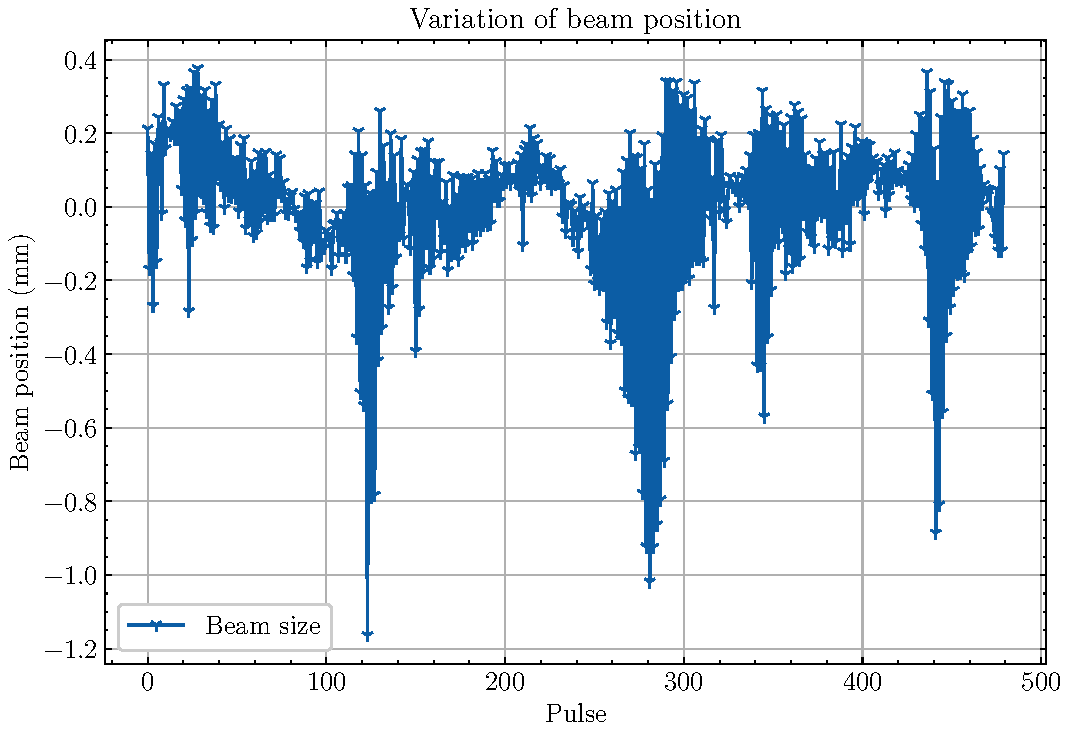
\includegraphics[width=1\textwidth]{04_Test/fig/fig000_variation_a}
      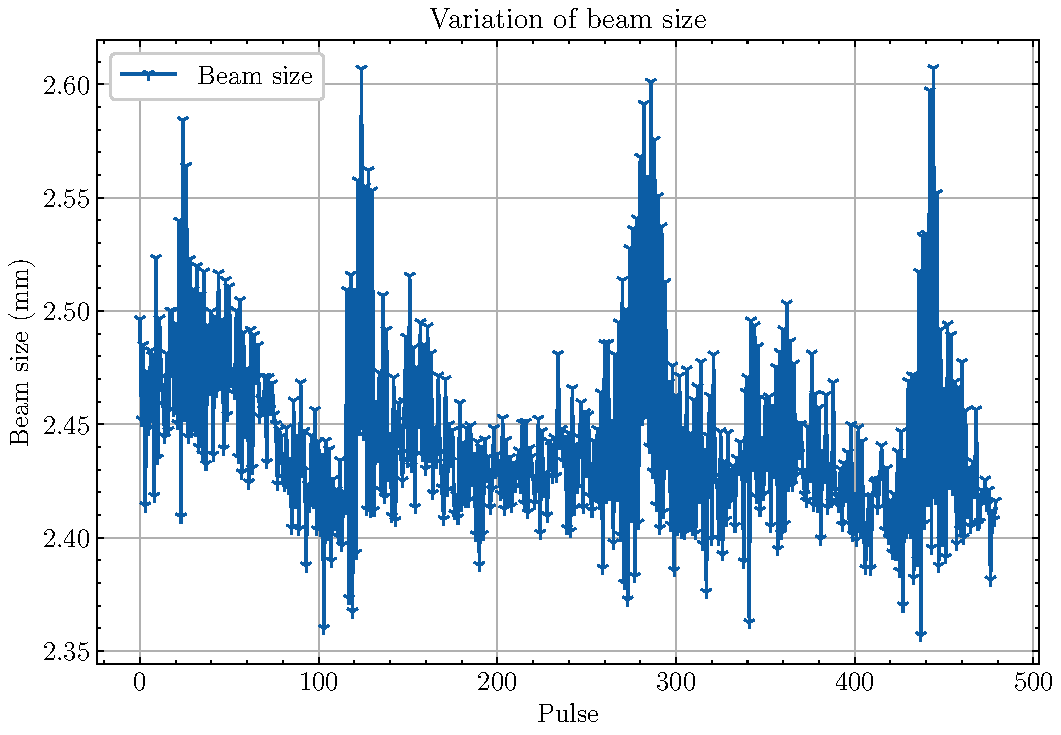
\includegraphics[width=1\textwidth]{04_Test/fig/fig000_variation_b}
    \end{column}
    \begin{column}{0.45\textwidth}
      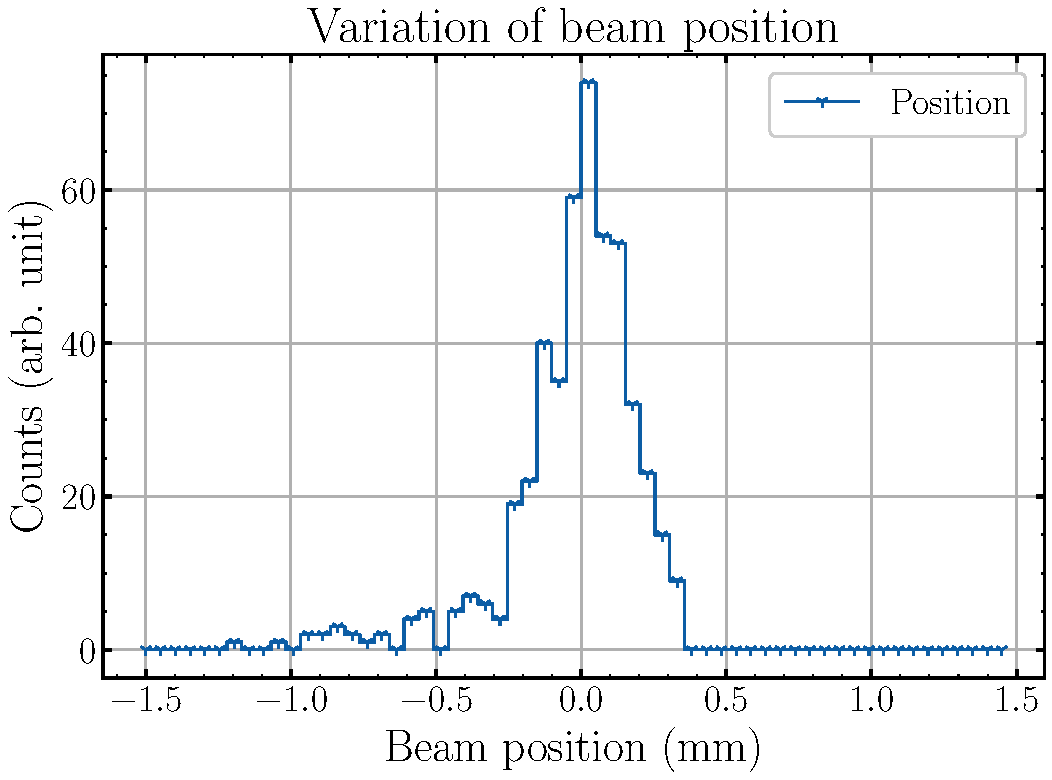
\includegraphics[width=1\textwidth]{04_Test/fig/fig000_hist_variation_a}
      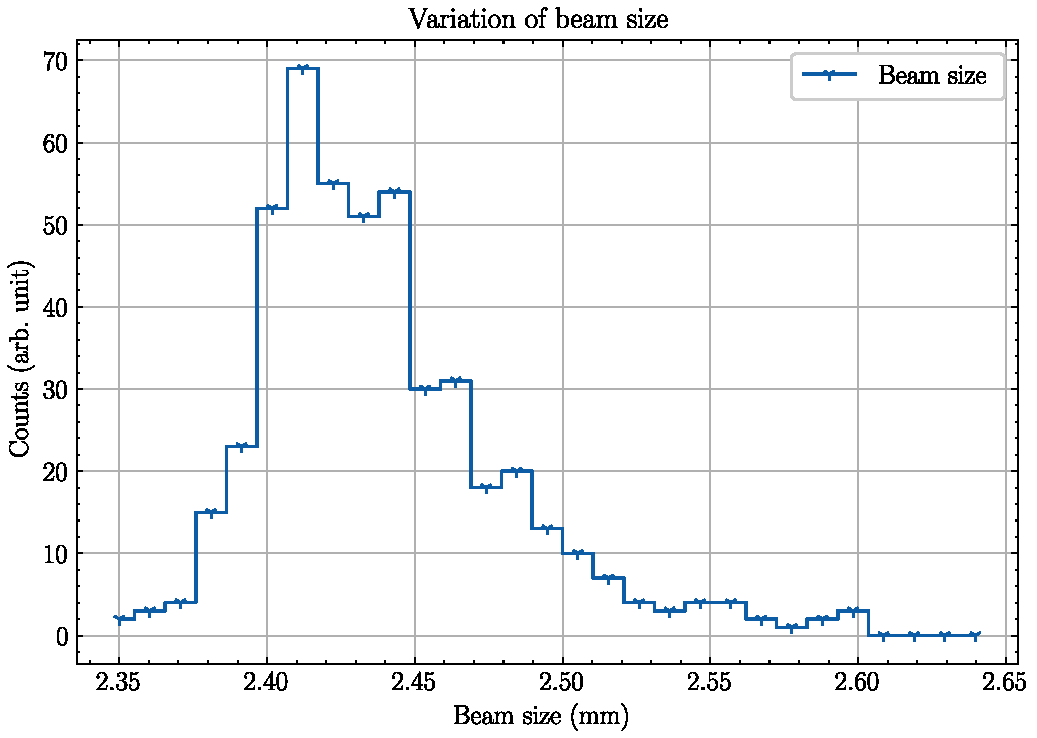
\includegraphics[width=1\textwidth]{04_Test/fig/fig000_hist_variation_b}
    \end{column}
  \end{columns}
\end{frame}

\begin{frame}[t]
  \frametitle{Beam conditions}
  \begin{columns}[T]
    \begin{column}{0.45\textwidth}
      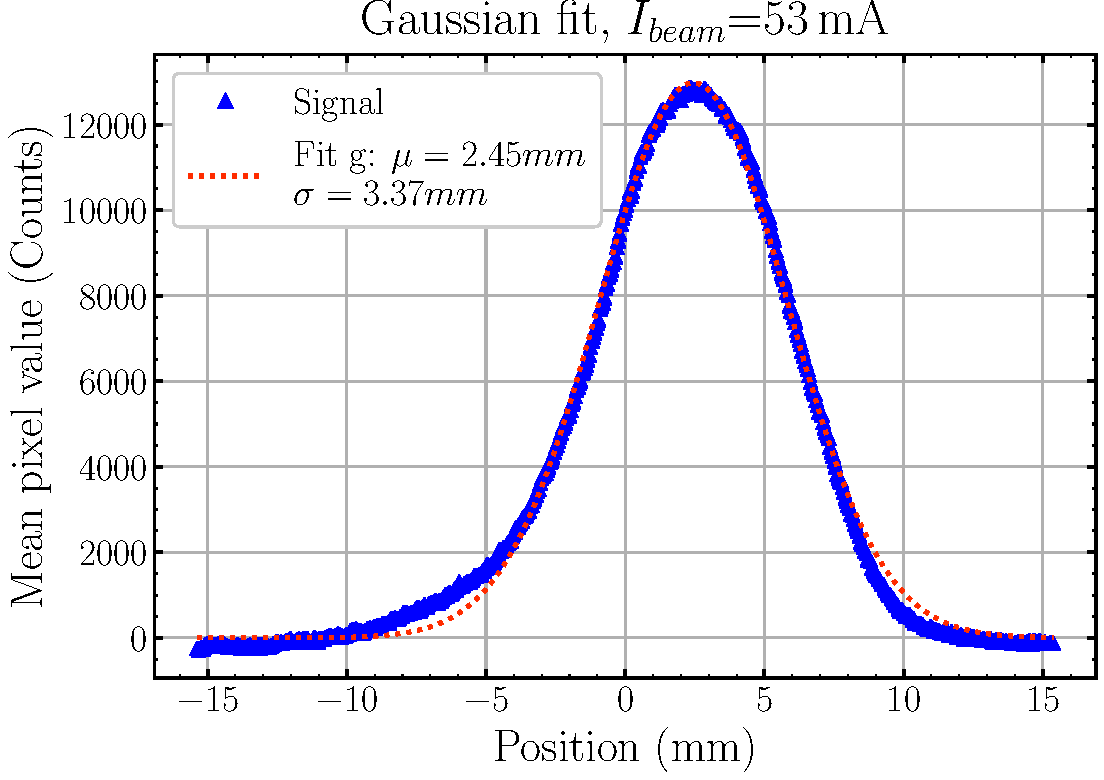
\includegraphics[width=1\textwidth]{04_Test/fig/fig000_ex_beam_profile_a3}
    \end{column}
    \begin{column}{0.45\textwidth}
      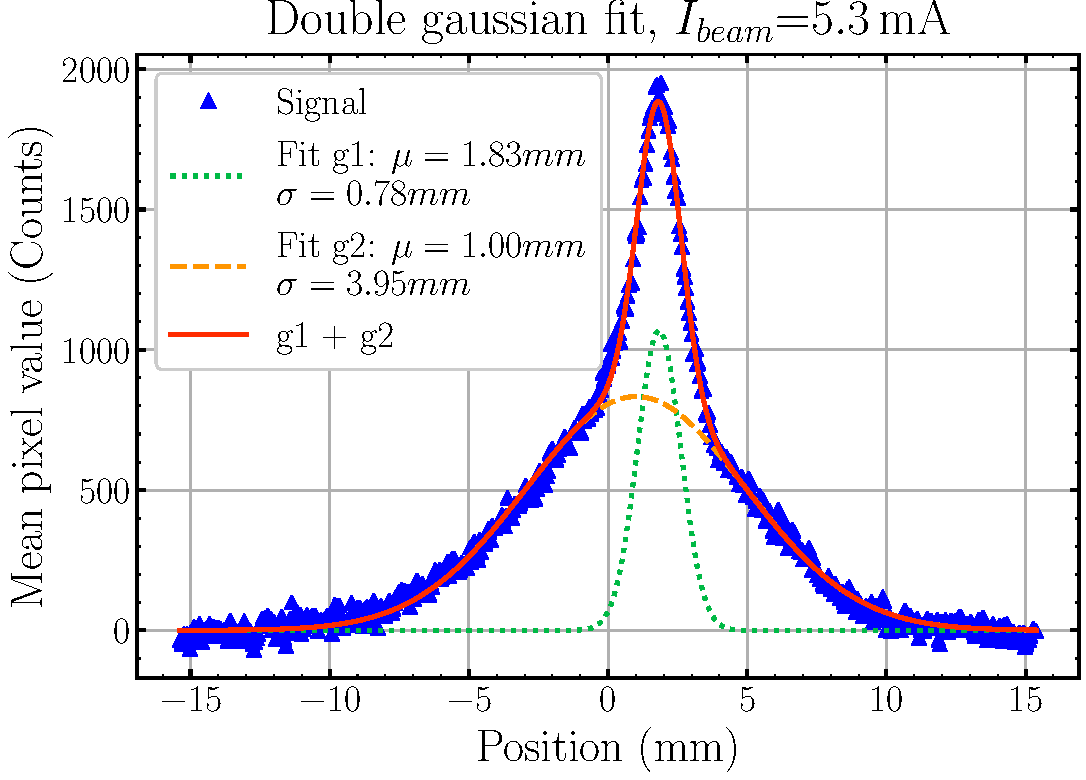
\includegraphics[width=1\textwidth]{04_Test/fig/fig000_ex_beam_profile_b3}
    \end{column}
  \end{columns}
  \begin{block}{Beam variations reduce the precision on measurement}
    \begin{itemize}
      \item Important position variation $\implies$ influence on size too.
      \item On 480 pulses:
            \begin{itemize}
              \item Position: Min-Max $\approx 1.6\,\mathrm{mm}$, $\sigma_{std} \approx 250\,\mathrm{\mu m}$
              \item Size: Min-Max $\approx 250\,\mathrm{\mu m}$, $\sigma_{std} \approx 50\,\mathrm{\mu m}$
            \end{itemize}
      \item Beam shape depends on current $\implies$ How to quantify size?
    \end{itemize}
  \end{block}
\end{frame}

% \begin{frame}[t]
%   \frametitle{Field uniformity}
%   \begin{alertblock}{}
%   \end{alertblock}
% \end{frame}

\begin{frame}[t]
  \frametitle{MCP system characterization}
  \begin{columns}[]
    \begin{column}{0.45\textwidth}
      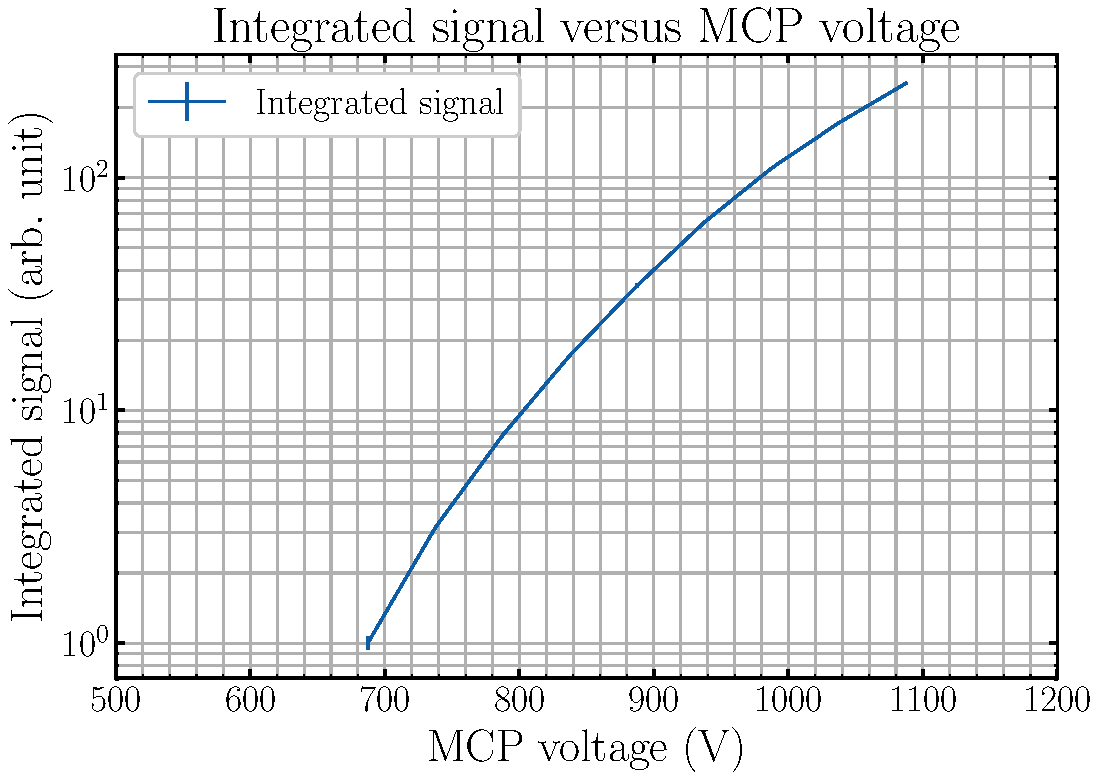
\includegraphics[width=1\textwidth]{04_Test/fig/fig000_MCP_gain_a}
      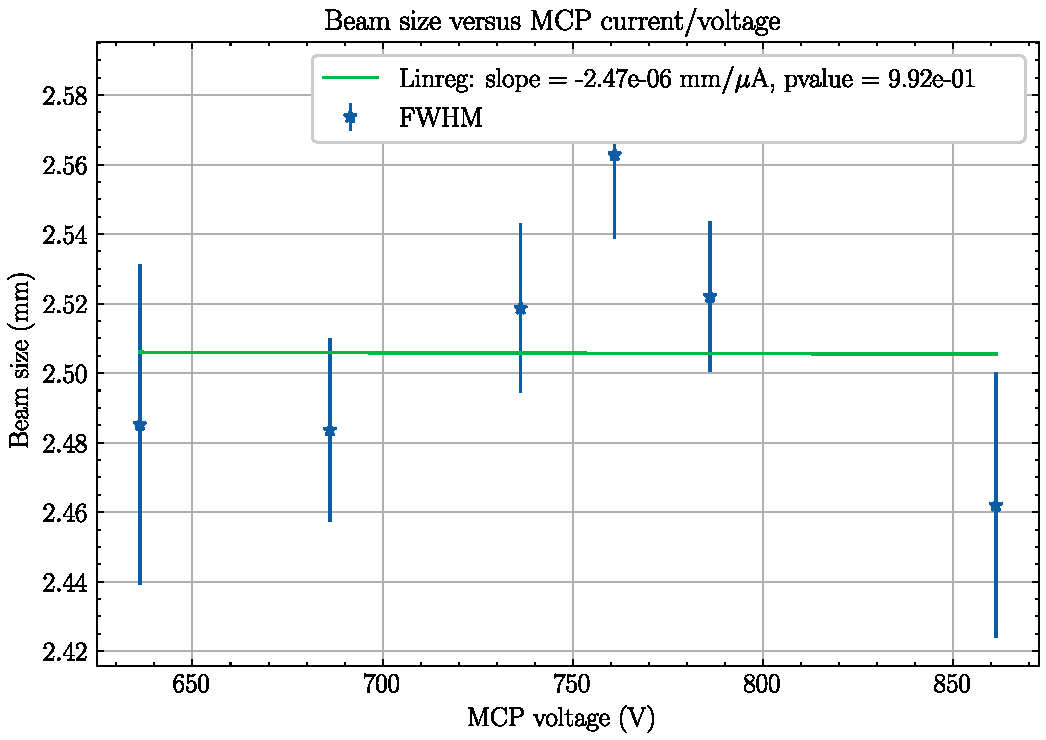
\includegraphics[width=1\textwidth]{04_Test/fig/fig000_MCP_gain_b}
    \end{column}

    \begin{column}{0.45\textwidth}
      \begin{block}{MCP is key component of the IPM}
        Gain: exponential

        Dynamic Range:
        \begin{itemize}
          \item Datasheet [600-1200V]:1000
          \item Tested [700-1100V]:300
        \end{itemize}

        Influence on beam size:
        \begin{itemize}
          \item Min-Max $\approx 100\,\mu m$
          \item Close to IPHI variations.
          \item Below ESS requirement.
        \end{itemize}
      \end{block}
    \end{column}
  \end{columns}
\end{frame}

\begin{frame}[t]
  \frametitle{Measurements with electrons}
  \centering
  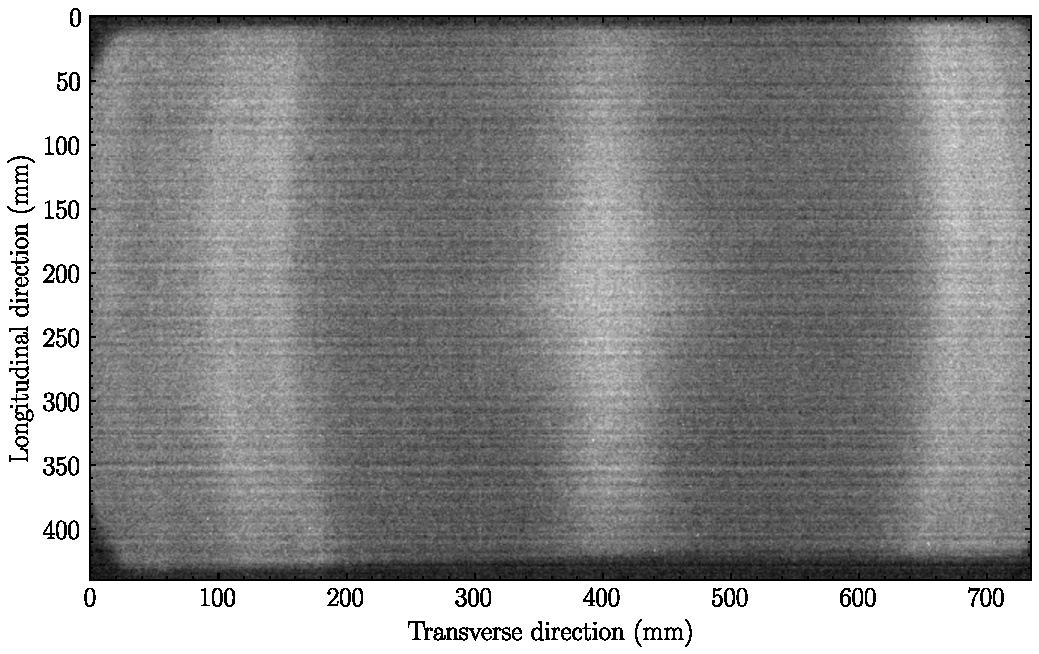
\includegraphics[width=0.7\textwidth]{04_Test/fig/fig000_electron_Photonis}
  \begin{block}{Impossible to get a profile with electrons at IPHI}
    \begin{itemize}
      \item Magnetic fields from devices like vacuum gauge.
      \item $e^-$ background?
    \end{itemize}
    Measurement is very difficult without guiding magnet.
  \end{block}
\end{frame}

\begin{frame}[t]
  \frametitle{Limits of detection}
  \begin{block}{An extrapolation to ESS conditions is assumed:}
    $Signal_{primary} \propto N_{beam}(I_{beam},t_{pulse}) \times \sigma_{ioniz.}(E_{beam},medium) \times \rho$
  \end{block}
  \begin{columns}[T]
    \begin{column}{0.35\textwidth}
      \begin{block}{Signal at IPHI is higher:}
        \begin{itemize}
          \item Lower beam energy
          \item Lower vacuum level
        \end{itemize}
        Factor: $5400$ at worst case and 1400 at best.
      \end{block}
    \end{column}
    \begin{column}{0.55\textwidth}
      \centering
      \includegraphics[width=1\textwidth]{04_Test/fig/fig000_Bethe_IPHI}
    \end{column}
  \end{columns}

  % \begin{columns}[T]
  %   \begin{column}{0.45\textwidth}
  %     \begin{block}{Limits with strips}
  %     \end{block}
  %   \end{column}
  %   \begin{column}{0.45\textwidth}

  %   \end{column}
  % \end{columns}
  \begin{alertblock}{But can be compensated by:}
    Reducing the beam current or the pulse duration.
  \end{alertblock}
\end{frame}

% \begin{frame}[t]
%   \frametitle{Limits of detection}
%   \begin{block}{Enough particle to reconstruct a profile?}
%     $Signal_{primary} = N_{beam}(I_{beam},t_{pulse}) \times \sigma_{proton}(E_{beam},medium,\rho)$
%   \end{block}
%   \begin{columns}[]
%     \begin{column}{0.35\textwidth}
%       \begin{block}{Signal at IPHI is higher:}
%         \begin{itemize}
%           \item Lower beam energy $\implies$ higher cross section
%           \item Lower vacuum level
%         \end{itemize}
%         But can be compensated by:
%         \begin{itemize}
%           \item Reducing the current
%           \item Reducing the pulse duration
%         \end{itemize}
%       \end{block}
%     \end{column}
%     \begin{column}{0.55\textwidth}
%       \centering
%       \includegraphics[width=1\textwidth]{04_Test/fig/fig000_Bethe_IPHI}
%     \end{column}
%   \end{columns}

%   \begin{columns}[T]
%     \begin{column}{0.45\textwidth}
%       \begin{block}{Limits with strips}
%       \end{block}
%     \end{column}
%     \begin{column}{0.45\textwidth}

%     \end{column}
%   \end{columns}
%   \begin{alertblock}{Conclusion}
%     Bare strips may not be able to detect at ESS.
%   \end{alertblock}
% \end{frame}

\begin{frame}[t]
  \frametitle{Limits of detection}
  \begin{columns}[T]
    \begin{column}{0.45\textwidth}
      \begin{block}{Limits with MCP}
        With MCP IPM $\rightarrow$ limits of IPHI:
        \begin{itemize}
          \item ESS: $62.5\,\mathrm{mA}$ and $2.86\,\mathrm{ms}$
          \item IPHI: $0.7\,\mathrm{mA}$ and $0.05\,\mathrm{ms}$
        \end{itemize}
      \end{block}
      The signal can be reduced by 5100 $\implies$ compensate the cross section.

      \begin{block}{Limits with strips}
        With strips IPM $\rightarrow$ limits of IPM:
        \begin{itemize}
          \item IPHI: $1.9\,\mathrm{mA}$ and $0.2\,\mathrm{ms}$
        \end{itemize}
      \end{block}
      The signal can be reduced by 500 $\implies$ and not compensate the cross section.

    \end{column}
    \begin{column}{0.45\textwidth}
      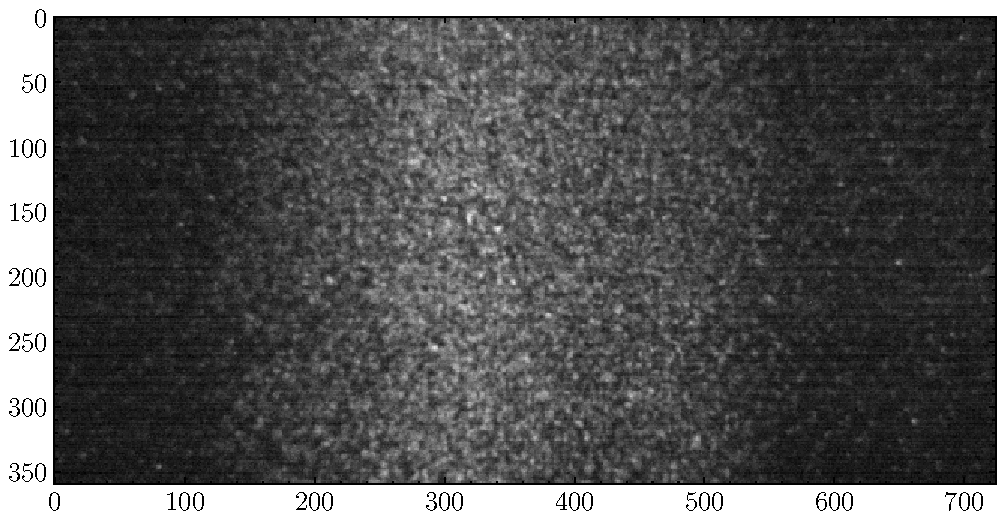
\includegraphics[width=1\textwidth]{04_Test/fig/fig000_limits_IPHI_a}
      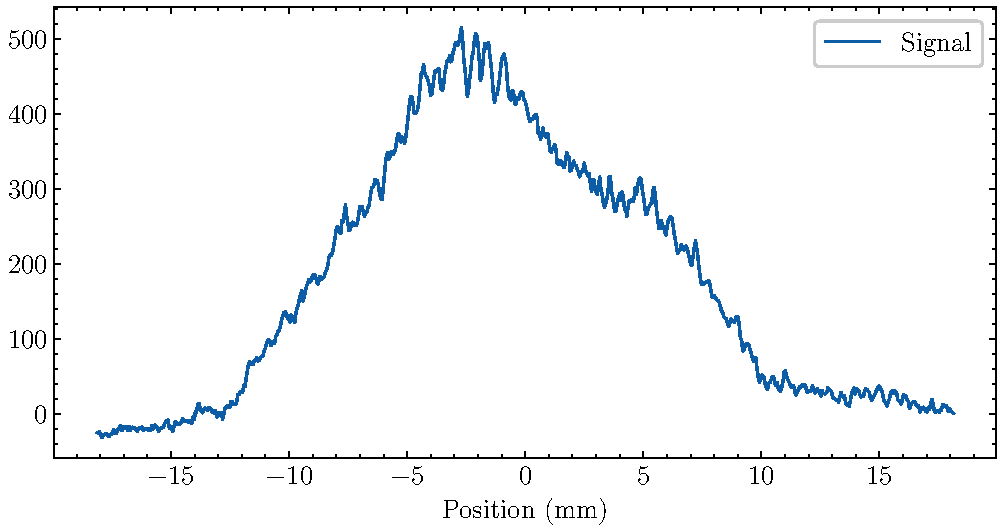
\includegraphics[width=1\textwidth]{04_Test/fig/fig000_limits_IPHI_b}
      \begin{alertblock}{Conclusion}
        Even a single stage MCP seems to be sufficient to detect profile.
        But bare strips are not sensitive enough for use at ESS.
      \end{alertblock}
    \end{column}
  \end{columns}
\end{frame}